\documentclass[12pt]{fphw}

\usepackage[utf8]{inputenc} % Required for inputting international characters
\usepackage[T1]{fontenc} % Output font encoding for international characters
\usepackage{mathpazo} % Use the Palatino font

\usepackage{graphicx} % Required for including images
\graphicspath{{./imgs}}

\usepackage{booktabs} % Required for better horizontal rules in tables

\usepackage{listings} % Required for insertion of code

\usepackage{enumerate} % To modify the enumerate environment

\usepackage{amsmath}
\usepackage{amssymb}
\usepackage{amsthm}

\title{Logic Coursework 2024/25: Written Work}
\author{Huseyin Emre Ozden}
\date{Tuesday, March 25th, 2025}
\institute{Durham University}
\class{Computational Thinking}
\professor{Prof. Barnaby Martin}

\begin{document}

\maketitle

\section*{Question 1}

\begin{problem}
  Answer the following questions about complete sets of logical connectives, in each case justifying your answer. \\
  (i) Show $\{\neg, \to \}$ is a complete set of connectives. \\
  (ii) Show $\{\to, 0\}$ is a complete set of connectives (where $0$ is the constant false). \\
  (iii) Is $\{ \text{NAND}, \wedge\}$ a complete set of connectives? \\
  (iv) Is $\{\wedge, \vee\}$ a complete set of connectives?
\end{problem}

\subsection*{Answer}

In order to determine whether the sets are complete, I will be showing whether $\wedge, \vee$ and $\neg$ can be expressed using the connectives in the set, in which case any logical expression can be written in CNF or DNF, meaning that it's a complete set.

\begin{proof}[Proof for part (i)] $ $ \newline
  Can $\vee$ be expressed using $\{\neg, \to \}$? \\
  Yes: $\neg p \to q \equiv \neg(\neg p) \vee q \equiv p \vee q$ \\
  Can $\wedge$ be expressed using $\{\neg, to \}$? \\
  Yes: $\neg(p \to \neg q) \equiv \neg (\neg p \vee \neg q) \equiv p \wedge q$ \\
  Since $\neg$ is already in our set of logical connectives, we can then conclude that $\{\neg, \to \}$ is a complete set of logical connectives, as any logical expression can be expressed in CNF/DNF using the connectives within the set.
\end{proof}

\begin{proof}[Proof for part (ii)] $ $ \newline
  Can $\neg$ be expressed using $\{\to, 0\}$? \\
  Yes: $p \to 0 \equiv \neg p \vee 0 \equiv \neg p$ \\
  Can $\vee$ be expressed using $\{\to, 0\}$? \\
  Yes: $(p \to 0) \to q \equiv \neg (p \to 0) \vee q \equiv \neg (\neg p ) \vee q \equiv p \vee q$ \\
  Can $\wedge$ be expressed using $\{\to, 0\}$? \\
  Yes: $(p \to (q \to 0)) \to 0 \equiv (p \to (\neg q \vee 0)) \to 0 \equiv (p \to \neg q) \to 0 \equiv (\neg p \vee \neg q) \to 0 \equiv \neg(\neg p \vee \neg q) \vee 0 \equiv p \wedge q$ \\
  Therefore $\{\to, 0\}$ is a complete set of logical connectives
\end{proof}

\begin{proof}[Proof for part (iii)] $ $ \newline
  To denote NAND, I will use the symbol: $\barwedge$ \\
  Can $\neg$ be expressed using $\{\barwedge, \wedge\}$? \\
  Yes: $p \barwedge p \equiv \neg(p \wedge p) \equiv \neg p$ \\
  Can $\vee$ be expressed using $\{\barwedge, \wedge\}$? \\
  Yes: $(p \barwedge p) \barwedge (q \barwedge q) \equiv \neg p \barwedge \neg q \equiv \neg(\neg p \wedge \neg q) \equiv p \vee q$ \\
  $\wedge$ is already in the set of logical connectives, therefore the set of logical connectives $\{\text{NAND}, \wedge\}$ is complete.
\end{proof}

\begin{proof}[Proof for part (iv)] $ $ \newline
  The set of logical connectives $\{\wedge, \vee\}$ is not complete as there is no way to represent one of the propositional variables being equal to zero (i.e: negation) when writing an expression in CNF/DNF. That is to say there is no way to express a tautology or contradiction using these logical connectives due to their property of idempotence.
\end{proof}
\section*{Question 2}

\begin{problem}
  Convert $(((p \to q) \to r) \to (s \to t))$ to \\
  (i) Conjunctive Normal Form (CNF) \\
  (ii) Disjunctive Normal Form (DNF)
\end{problem}

\subsection*{Answer}

\ \newline
This question is easier to approach by writing the expression $\varphi = (((p \to q) \to r) \to (s \to t))$ in DNF first:
\begin{gather*}
  \varphi \equiv (((\neg p \vee q) \to r) \to (s \to t)) \\
  \equiv ((\neg(\neg p \vee q) \vee r) \to (s \to t)) \\
  \equiv (((p \wedge \neg q) \vee r) \to (s \to t)) \\
  \equiv (\neg((p \wedge \neg q) \vee r) \vee (s \to t)) \\
  \equiv ((\neg(p \wedge \neg q) \wedge \neg r) \vee (s \to t)) \\
  \equiv (((\neg p \vee q) \wedge \neg r) \vee (s \to t)) \\
  \equiv (((\neg p \wedge \neg r) \vee (q \wedge \neg r)) \vee (s \to t)) \\
  \equiv ((\neg p \wedge \neg r) \vee (q \wedge \neg r) \vee (\neg s \vee t)) \\
  \equiv (\neg p \wedge \neg r) \vee (q \wedge \neg r) \vee \neg s \vee t \\
  \therefore \varphi_{DNF} = (\neg p \wedge \neg r) \vee (q \wedge \neg r) \vee \neg s \vee t
\end{gather*}

Using this, we can repeatedly use the distributive property to convert this to conjunctive normal form:

\begin{gather*}
  \varphi_{DNF} = (\neg p \wedge \neg r) \vee (q \wedge \neg r) \vee \neg s \vee t \\
  \equiv ((\neg p \vee q) \wedge \neg r) \vee \neg s \vee t \\
  \equiv (((\neg p \vee q) \vee \neg s) \wedge (\neg r \vee \neg s)) \vee t \\
  \equiv (\neg p \vee q \vee \neg s \vee t) \wedge (\neg r \vee \neg s \vee t) \\
  \therefore \varphi_{CNF} = (\neg p \vee q \vee \neg s \vee t) \wedge (\neg r \vee \neg s \vee t)
\end{gather*}

(i) $\varphi_{CNF} = (\neg p \vee q \vee \neg s \vee t) \wedge (\neg r \vee \neg s \vee t)$

(ii) $\varphi_{DNF} =(\neg p \wedge \neg r) \vee (q \wedge \neg r) \vee \neg s \vee t$

\newpage

\section*{Question 3}

\begin{problem}
  What is the purpose of Tseitin's Algorithm? Apply Tseitin's Algorithm to turn the propositional formula $(((x_1 \wedge x_2 \wedge x_3) \to (y_1 \wedge y_2 \wedge y_3)) \vee z)$ to CNF.
\end{problem}

\subsection*{Answer} \ \newline
The purpose of Tseitin's Algorithm is to take an arbitrary propositional formula $\varphi$, and transform it to a new propositional formula $\varphi'$ which is equisatisfiable with $\varphi$, and in conjunctive normal form.
\begin{gather*}
  \text{Let } \varphi = (((x_1 \wedge x_2 \wedge x_3) \to (y_1 \wedge y_2 \wedge y_3)) \vee z) \\
  \text{Introduce new variables for each subformula:} \\
  \alpha_1 \leftrightarrow x_1 \wedge x_2 \wedge x_3 \\
  \alpha_2 \leftrightarrow y_1 \wedge y_2 \wedge y_3 \\
  \alpha_3 \leftrightarrow \alpha_1 \to \alpha_2 \\
  \alpha_4 \leftrightarrow \alpha_3 \vee z \\
  \text{Write each expression as conjunctions} \\
  \text{From } \alpha_1: \\
  \alpha_1 \leftrightarrow (x_1 \wedge x_2 \wedge x_3) \equiv (\alpha_1 \to (x_1 \wedge x_2 \wedge x_3)) \wedge (\alpha_1 \leftarrow (x_1 \wedge x_2 \wedge x_3)) \\
  \equiv (\neg \alpha_1 \vee (x_1 \wedge x_2 \wedge x_3)) \wedge (\alpha_1 \vee \neg(x_1 \wedge x_2 \wedge x_3)) \\
  \equiv (\neg \alpha_1 \vee x_1) \wedge (\neg \alpha_1 \vee x_2) \wedge (\neg \alpha_1 \vee x_3) \wedge (\alpha_1 \vee \neg x_1 \vee \neg x_2 \vee \neg x_3) \\
  \text{Similarly for } \alpha_2: \\
  \alpha_2 \leftrightarrow (y_1 \wedge y_2 \wedge y_3) \equiv (\neg \alpha_2 \vee y_1) \wedge (\neg \alpha_2 \vee y_2) \wedge (\neg \alpha_2 \vee y_3) \wedge (\alpha_2 \vee \neg y_1 \vee \neg y_2 \vee \neg y_3) \\
  \text{For } \alpha_3: \\ 
  \alpha_3 \leftrightarrow (\alpha_1 \to \alpha_2) \equiv (\alpha_3 \to (\alpha_1 \to \alpha_2)) \wedge (\alpha_3 \leftarrow (\alpha_1 \to \alpha_2))\\ 
  \equiv (\neg \alpha_3 \vee (\neg \alpha_1 \vee \alpha_2)) \wedge (\neg(\neg \alpha_1 \vee \alpha_2) \vee \alpha_3)  \equiv (\neg \alpha_3 \vee \neg \alpha_1 \vee \alpha_2) \wedge ((\alpha_1 \wedge \neg \alpha_2) \vee \alpha_3) \\
  \equiv (\neg \alpha_1 \vee \alpha_2 \vee \neg \alpha_3) \wedge (\alpha_1 \vee \alpha_3) \wedge (\neg \alpha_2 \vee \alpha_3) \\
  \text{For } \alpha_4: \\
  \alpha_4 \leftrightarrow (\alpha_3 \vee z) \equiv (\alpha_4 \to (\alpha_3 \vee z)) \wedge (\alpha_4 \leftarrow (\alpha_3 \vee z)) \\ 
  \equiv (\neg \alpha_4 \vee \alpha_3 \vee z) \wedge (\neg (\alpha_3 \vee z) \vee \alpha_4) \equiv (\neg \alpha_4 \vee \alpha_3 \vee z) \wedge ((\neg \alpha_3 \wedge \neg z) \vee \alpha_4) \\
  \equiv (\neg \alpha_4 \vee \alpha_3 \vee z) \wedge (\neg \alpha_3 \vee \alpha_4) \wedge (\neg z \vee \alpha_4) \\
  \text{The conjunction of all these variables and the clause } \alpha_4 \\
  \text{ gives us the Tseitin Transformation of } \varphi' \\
  \text{To save space, I will write this as a clause set} \\
  \therefore \varphi' = \{\{\alpha_4\}, \{-\alpha_1, x_1\}, \{-\alpha_1, x_2\}, \{-\alpha_1, x_3\}, \{\alpha_1, -x_1, -x_2, -x_3\}, \\ \{-\alpha_2, y_1\}, \{-\alpha_2, y_2\}, \{-\alpha_2, y_3\}, \{\alpha_2, -y_1, -y_2, -y_3\}, \\ \{-\alpha_1, \alpha_2, -\alpha_3\}, \{\alpha_1, \alpha_3\}, \{-\alpha_2, \alpha_3\}, \{-\alpha_4, \alpha_3, z\}, \{-\alpha_3, \alpha_4\}, \{-z, \alpha_4\}\}
\end{gather*}

\section*{Question 4}

\begin{problem}
  State with justification if each of the following sentences of predicate logic is logically valid. \\
  (i) $(\forall x \exists y \forall z (E(x,y) \wedge E(y,z))) \to (\forall x \forall z \exists y (E(x,y) \wedge E(y,z)))$ \\
  (ii) $(\forall x \exists y \exists u \forall v (E(x,y) \wedge E(u,v))) \to (\exists u \forall v \forall x \exists y (E(x,y) \wedge E(u,v)))$ \\
  (iii) $(\forall x \exists y \forall z \ R(x,y,z)) \to (\exists x \forall y \exists z \ R(x,y,z))$ \\
  (iv) $(\forall x \forall y \exists z (E(x,y) \wedge E(y,z))) \to (\forall x \forall y \forall z (E(x,y) \vee E(y,z)))$
\end{problem}

\subsection*{Answer} \ \newline
(i) Logically Valid.
\begin{proof}
    In both the antecedent and consequent, $x$ and $y$ are quantified in the same order, so $E(x,y)$ is true in both cases. It also follows that if there exists a $y$, for all values of $z$, such that $E$ holds then it is sufficient that for all $z$, there exists a $y$, such that $E$ holds.
    Therefore it follows that this sentence is logically valid.
\end{proof}  \noindent
(ii) Logically Valid.
\begin{proof}
    We can begin by considering an interpretation $I$:
    \begin{gather*}
        I \models \forall x \exists y \exists u \forall v (E(x,y) \wedge E(u,v)) \iff I \models \forall x \exists y E(x,y) \wedge \exists u \forall v E(u, v) \\ 
        \iff I \models \exists u \forall v \forall x \exists y (E(x,y) \wedge E(u,v))
    \end{gather*}
    Hence it follows that $\forall x \exists y \exists u \forall v (E(x,y) \wedge E(u,v)) \equiv \exists u \forall v \forall x \exists y(E(x,y) \wedge E(u,v))$. Since the antecedent and consequent are logically equivalent, it follows that this sentence is a tautology, therefore logically valid.
\end{proof} \noindent
(iii) Logically Invalid.
\begin{proof}
In order to demonstrate that this is a logically invalid sentence, I will provide a counter-model: Consider $R$ a terenary relation over the domain $\{0, 1\}$, where
$$
R := \{(0,0,0),(0,0,1),(1,0,0),(1,0,1)\}
$$
From this we can see, that for all values of $x$, there in fact is a $y$, for all $z$. However there doesn't exist an $x$ for all values of $y$, where there exists a $z$. This is because $y$ only appears as a $0$ in the relation, hence $y$ cannot take each value in the domain in this relation.
\end{proof} \noindent
(iv) Logically Valid.
\begin{proof}
    Let's re-write the equation by re-arranging the quantifiers as such:
    \begin{gather*}
        \forall x \forall y \exists z (E(x,y) \wedge E(y,z)) \to \forall x \forall y \forall z (E(x,y) \wedge E(y,z)) \\ 
        \equiv \forall y (\forall x E(x,y) \wedge \exists z E(y,z)) \to \forall y (\forall x E(x,y) \vee \forall z E(y,z))
    \end{gather*}
    For the antecedent to hold true, we require both $\forall x E(x,y)$ and $\exists z E(y,z)$ to hold true. Therefore if the antecedent is true, then $\forall x E(x,y)$ must be true, which means then that the $\forall x E(x,y)$ in the consequent must also hold true. Therefore this sentence is logically valid.
\end{proof} \noindent

\section*{Question 5}

\begin{problem}
  Evaluate the given sentence on the respective relation $E$ over domain $\{0,1,2\}$ with relation $E := \{(0,1),(1,0),(1,2),(2,1),(2,0),(0,2)\}$\\ \\
  (i) $\forall x \forall y \forall z \exists w (E(x,w) \wedge E(y,w) \wedge E(z,w))$ \\
  (ii) $\exists x \forall y \forall z \exists w (E(x,w) \wedge E(y,w) \wedge E(z,w))$ \\
  (iii) $\forall y \exists x \forall z \exists w (E(x,w) \wedge E(y,w) \wedge E(z,w))$ \\
  (iv) $\exists x \exists y \exists z \forall w (E(x,w) \wedge E(y,w) \wedge E(z,w))$ \\
  (v) $\forall x_1 \exists x_2 \forall y_1 \exists y_2 \forall z_1 \exists z_2 \forall z \exists w \ E(x_1, x_2) \wedge E(x_2, w) \wedge E(y_1, y_2) \wedge E(y_2, w) \wedge E(z_1, z_2) \wedge E(z_2, w) \wedge E(z,w)$ \\
  (vi) $\forall x_1 \exists x_2 \forall y_1 \exists y_2 \forall z_1 \forall z \exists z_2 \exists w \ E(x_1, x_2) \wedge E(x_2, w) \wedge E(y_1, y_2) \wedge E(y_2, w) \wedge E(z_1, z_2) \wedge E(z_2, w) \wedge E(z,w)$
\end{problem}

\subsection*{Answer} \ \newline
For the purposes of this question, it will be easier to express the relation $E$ as such:
$$
E := \{(u,v) \in \{0,1,2\} : u \neq v \}
$$
(i) False. This sentence can be refuted by assigning the following variables:
$$
x = 0, y = 1, z = 2
$$
That is to say, the expression inside the brackets requires that $x \neq w, y \neq w, z \neq w$. However if we assign $x,y,z$ uniquely, by the pigeonhole principle, it follows that there will exist no such $w$, that satisfies the sentence. \newline \newline
(ii) False. This sentence can be refuted by considering the fact that if $x, y, z$ are unique, then there will exist no $w$, such that the conjunction of the atomic formulae $E(x,w), E(y,w), E(z,w)$ are satisfied. From the domain of the interpretation, we can deduce that there is no such value of $x$. \newline \newline
For the most part of the rest of this question, it will be easier to visualize the interpretation as a graph:
\begin{center}
    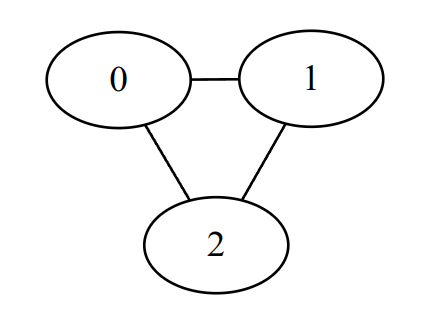
\includegraphics[scale=0.5]{q5-graph.png}
\end{center}
Where an edge on the graph represents the unordered pairs of numbers in the defined domain. \newline \newline
(iii) True. The sentence $\forall y \exists x \forall z \exists w (E(x,w) \wedge E(y,w) \wedge E(z,w))$ can be demonstrated to hold true, as for all y, if we choose the $x$, such that $x = y$, then for all values of $z$, it will follow that there will always exist a $w$ that is not already picked on the graph \newline \newline
(iv) True. In this interpretation, for the sentence to be true, there must exist $x,y,z$ for all $w$, such that none of $x,y,z$ is equal to $w$. It then becomes clear that for each $w$, we can choose $x,y,z$ such that $x=y$ or $x = z$ or $y = z$ and $x,y,z \neq w$.\newline \newline
(v) False.  If we assign $x_1,y_1,z_1$ uniquely, then there will be adjacent vertices $x_2,y_2,z_2$, where 2 of the 3 variables $x_2,y_2,z_2$ must be the same. For the sentence to hold, all $x_2,y_2,z_2, z$ there must exist an adjacent node $w$. However, if $x_2$, $y_2$ and $z_2$ are unique, for all values of $z$ there will be no $w$ such that the expression is satisfied.   \newline \newline
(vi) False. Although this is similar to the previous question, in that if the previous question were to hold true, then the answer to this question would also follow. However since it is in fact not true, it is not necessary that the conclusion of this sentence is the same as the previous one. If we assign $x_1$ and an adjacent $x_2$, do the same for $y_1$ and $y_2$, and then assign $z_1$, where $z_1 \neq y_1 \neq x_1$. If $y_2$ and $x_2$ are both assigned uniquely, when we assign $z$ and $z_2$, where once again $z_2 \neq y_2 \neq x_1$, then no value of $w$ will satisfy the equation. \newline \newline
\end{document}